

\tikzset{every picture/.style={line width=0.75pt}} %set default line width to 0.75pt        

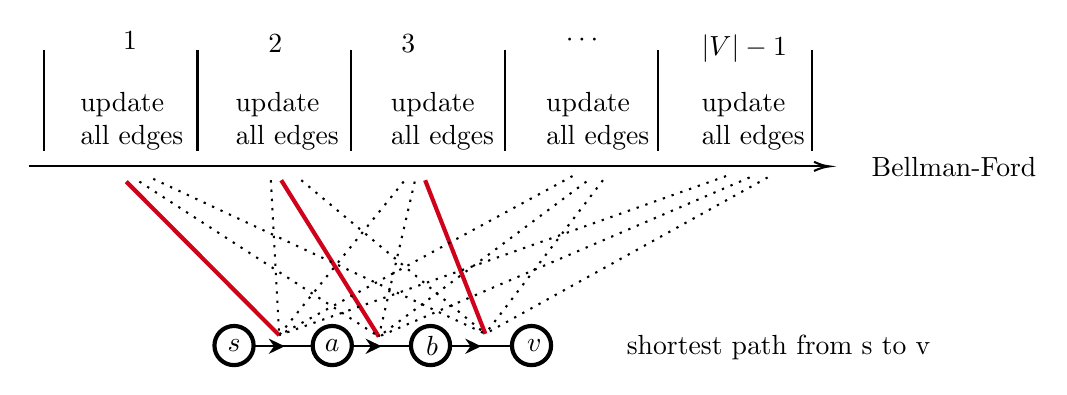
\begin{tikzpicture}[x=0.5pt,y=0.5pt,yscale=-1,xscale=1]
%uncomment if require: \path (0,293); %set diagram left start at 0, and has height of 293

%Straight Lines [id:da42563372855460047] 
\draw [color={rgb, 255:red, 0; green, 0; blue, 0 }  ,draw opacity=1 ][line width=0.75]    (250.5,248) -- (293.5,248) ;
\draw [shift={(272,248)}, rotate = 180] [fill={rgb, 255:red, 0; green, 0; blue, 0 }  ,fill opacity=1 ][line width=0.08]  [draw opacity=0] (11.61,-5.58) -- (0,0) -- (11.61,5.58) -- (7.71,0) -- cycle    ;
%Straight Lines [id:da13574797376852343] 
\draw [color={rgb, 255:red, 0; green, 0; blue, 0 }  ,draw opacity=1 ][line width=0.75]    (322.5,248) -- (365.5,248) ;
\draw [shift={(344,248)}, rotate = 180] [fill={rgb, 255:red, 0; green, 0; blue, 0 }  ,fill opacity=1 ][line width=0.08]  [draw opacity=0] (11.61,-5.58) -- (0,0) -- (11.61,5.58) -- (7.71,0) -- cycle    ;
%Straight Lines [id:da9930965641121888] 
\draw    (17,118) -- (593.5,118) ;
\draw [shift={(595.5,118)}, rotate = 180] [color={rgb, 255:red, 0; green, 0; blue, 0 }  ][line width=0.75]    (10.93,-3.29) .. controls (6.95,-1.4) and (3.31,-0.3) .. (0,0) .. controls (3.31,0.3) and (6.95,1.4) .. (10.93,3.29)   ;
%Straight Lines [id:da09874107164515367] 
\draw [color={rgb, 255:red, 0; green, 0; blue, 0 }  ,draw opacity=1 ][line width=0.75]    (180.5,248) -- (223.5,248) ;
\draw [shift={(202,248)}, rotate = 180] [fill={rgb, 255:red, 0; green, 0; blue, 0 }  ,fill opacity=1 ][line width=0.08]  [draw opacity=0] (11.61,-5.58) -- (0,0) -- (11.61,5.58) -- (7.71,0) -- cycle    ;
%Straight Lines [id:da6519777460675502] 
\draw [color={rgb, 255:red, 208; green, 2; blue, 27 }  ,draw opacity=1 ][line width=1.5]    (198,240) -- (87.5,129) ;
%Straight Lines [id:da29298485524387174] 
\draw [color={rgb, 255:red, 208; green, 2; blue, 27 }  ,draw opacity=1 ][line width=1.5]    (270,241) -- (199.5,128) ;
%Straight Lines [id:da3208602618624562] 
\draw [color={rgb, 255:red, 208; green, 2; blue, 27 }  ,draw opacity=1 ][line width=1.5]    (347,239) -- (303.5,128) ;
%Straight Lines [id:da3600584205418621] 
\draw    (139,34) -- (139,107) ;
%Straight Lines [id:da02657749763727446] 
\draw    (250,34) -- (250,107) ;
%Straight Lines [id:da432596125208347] 
\draw    (361,34) -- (361,107) ;
%Straight Lines [id:da23108993646686993] 
\draw    (472,34) -- (472,107) ;
%Straight Lines [id:da4614439049417304] 
\draw    (583,34) -- (583,107) ;
%Straight Lines [id:da16560659557639468] 
\draw    (28,34) -- (28,107) ;
%Straight Lines [id:da25208194451529387] 
\draw  [dash pattern={on 0.84pt off 2.51pt}]  (192,128) -- (198,240) ;
%Straight Lines [id:da7861583212855291] 
\draw  [dash pattern={on 0.84pt off 2.51pt}]  (288,129) -- (198,240) ;
%Straight Lines [id:da49185141998689486] 
\draw  [dash pattern={on 0.84pt off 2.51pt}]  (410,125) -- (198,240) ;
%Straight Lines [id:da8179307613761421] 
\draw  [dash pattern={on 0.84pt off 2.51pt}]  (521,125) -- (198,240) ;
%Straight Lines [id:da738826011238115] 
\draw  [dash pattern={on 0.84pt off 2.51pt}]  (97,129) -- (270,241) ;
%Straight Lines [id:da7922029908645758] 
\draw  [dash pattern={on 0.84pt off 2.51pt}]  (296,129) -- (270,241) ;
%Straight Lines [id:da17863430138132286] 
\draw  [dash pattern={on 0.84pt off 2.51pt}]  (420,129) -- (270,241) ;
%Straight Lines [id:da1994756861969148] 
\draw  [dash pattern={on 0.84pt off 2.51pt}]  (538,126) -- (270,241) ;
%Straight Lines [id:da15961835119738887] 
\draw  [dash pattern={on 0.84pt off 2.51pt}]  (107,127) -- (347,239) ;
%Straight Lines [id:da2160261066023147] 
\draw  [dash pattern={on 0.84pt off 2.51pt}]  (214,128) -- (347,239) ;
%Straight Lines [id:da11926591660202601] 
\draw  [dash pattern={on 0.84pt off 2.51pt}]  (432,128) -- (347,239) ;
%Straight Lines [id:da3590914844591715] 
\draw  [dash pattern={on 0.84pt off 2.51pt}]  (551,126) -- (347,239) ;

% Text Node
\draw  [line width=1.5]   (165.38, 247.47) circle [x radius= 14.15, y radius= 14.15]   ;
\draw (165.38,247.47) node   [align=left] {$\displaystyle s$};
% Text Node
\draw  [line width=1.5]   (236.38, 247.47) circle [x radius= 14.15, y radius= 14.15]   ;
\draw (236.38,247.47) node   [align=left] {$\displaystyle a$};
% Text Node
\draw  [line width=1.5]   (307.38, 247.47) circle [x radius= 14.15, y radius= 14.15]   ;
\draw (301.88,247.47) node [anchor=west] [inner sep=0.75pt]   [align=left] {$\displaystyle b$};
% Text Node
\draw  [line width=1.5]   (380.38, 247.47) circle [x radius= 14.15, y radius= 14.15]   ;
\draw (374.88,247.47) node [anchor=west] [inner sep=0.75pt]   [align=left] {$\displaystyle v$};
% Text Node
\draw (624,109) node [anchor=north west][inner sep=0.75pt]   [align=left] {Bellman-Ford};
% Text Node
\draw (447,238) node [anchor=north west][inner sep=0.75pt]   [align=left] {shortest path from s to v};
% Text Node
\draw (52,62) node [anchor=north west][inner sep=0.75pt]   [align=left] {update\\all edges};
% Text Node
\draw (164.25,62) node [anchor=north west][inner sep=0.75pt]   [align=left] {update\\all edges};
% Text Node
\draw (276.5,62) node [anchor=north west][inner sep=0.75pt]   [align=left] {update\\all edges};
% Text Node
\draw (388.75,62) node [anchor=north west][inner sep=0.75pt]   [align=left] {update\\all edges};
% Text Node
\draw (501,62) node [anchor=north west][inner sep=0.75pt]   [align=left] {update\\all edges};
% Text Node
\draw (74,20.5) node [anchor=north west][inner sep=0.75pt]   [align=left] {$ $};
% Text Node
\draw (188,20.5) node [anchor=north west][inner sep=0.75pt]   [align=left] {$\displaystyle 2$};
% Text Node
\draw (284,20.5) node [anchor=north west][inner sep=0.75pt]   [align=left] {$\displaystyle 3$};
% Text Node
\draw (403,20.5) node [anchor=north west][inner sep=0.75pt]   [align=left] {$\displaystyle \cdots $};
% Text Node
\draw (501,20.5) node [anchor=north west][inner sep=0.75pt]   [align=left] {$\displaystyle |V|-1$};
% Text Node
\draw (83,18.5) node [anchor=north west][inner sep=0.75pt]   [align=left] {$\displaystyle 1$};


\end{tikzpicture}

